\documentclass[12pt, a4paper]{article}

% ── Packages ──
\usepackage[margin=1in]{geometry}
\usepackage{amsmath, amssymb, amsfonts}
\usepackage{booktabs}
\usepackage{graphicx}
\usepackage{xcolor}
\usepackage{tikz}
\usetikzlibrary{calc, positioning, arrows.meta, shapes.geometric, decorations.pathreplacing, matrix}
\usepackage{tcolorbox}
\tcbuselibrary{skins, breakable}
\usepackage{enumitem}
\usepackage{hyperref}
\usepackage{fancyhdr}
\usepackage{titlesec}
\usepackage{colortbl}
\usepackage{multirow}
\usepackage{array}
\usepackage{float}
\usepackage{pifont}

% ── Colors ──
\definecolor{darkblue}{HTML}{1a365d}
\definecolor{medblue}{HTML}{2b6cb0}
\definecolor{lightblue}{HTML}{ebf8ff}
\definecolor{darkgreen}{HTML}{276749}
\definecolor{lightgreen}{HTML}{f0fff4}
\definecolor{darkred}{HTML}{9b2c2c}
\definecolor{lightred}{HTML}{fff5f5}
\definecolor{darkorange}{HTML}{c05621}
\definecolor{lightorange}{HTML}{fffaf0}
\definecolor{darkpurple}{HTML}{553c9a}
\definecolor{lightpurple}{HTML}{faf5ff}
\definecolor{darkteal}{HTML}{285e61}
\definecolor{lightteal}{HTML}{e6fffa}
\definecolor{tp_green}{HTML}{48bb78}
\definecolor{fp_red}{HTML}{fc8181}
\definecolor{fn_orange}{HTML}{f6ad55}
\definecolor{tn_blue}{HTML}{63b3ed}

% ── tcolorbox styles ──
\newtcolorbox{keyidea}[1][]{
    colback=lightblue, colframe=medblue, fonttitle=\bfseries,
    title=#1, rounded corners, boxrule=1pt, breakable
}
\newtcolorbox{warningbox}[1][]{
    colback=lightred, colframe=darkred, fonttitle=\bfseries,
    title=#1, rounded corners, boxrule=1pt, breakable
}
\newtcolorbox{examplebox}[1][]{
    colback=lightgreen, colframe=darkgreen, fonttitle=\bfseries,
    title=#1, rounded corners, boxrule=1pt, breakable
}
\newtcolorbox{intuitionbox}[1][]{
    colback=lightorange, colframe=darkorange, fonttitle=\bfseries,
    title=#1, rounded corners, boxrule=1pt, breakable
}
\newtcolorbox{formulabox}[1][]{
    colback=lightpurple, colframe=darkpurple, fonttitle=\bfseries,
    title=#1, rounded corners, boxrule=1pt, breakable
}
\newtcolorbox{summarybox}[1][]{
    colback=lightteal, colframe=darkteal, fonttitle=\bfseries,
    title=#1, rounded corners, boxrule=1pt, breakable
}

% ── Header/Footer ──
\pagestyle{fancy}
\fancyhf{}
\fancyhead[L]{\small\textcolor{darkblue}{Evaluation Metrics --- Explained}}
\fancyhead[R]{\small\textcolor{darkblue}{Thesis Reference Guide}}
\fancyfoot[C]{\thepage}
\renewcommand{\headrulewidth}{0.5pt}

% ── Section formatting ──
\titleformat{\section}{\LARGE\bfseries\color{darkblue}}{}{0em}{}[\vspace{-0.5em}\textcolor{medblue}{\rule{\textwidth}{1pt}}]
\titleformat{\subsection}{\Large\bfseries\color{medblue}}{}{0em}{}

% ── Document ──
\begin{document}

% ══════════════════════════════════════════════════════════════
%                        TITLE PAGE
% ══════════════════════════════════════════════════════════════
\begin{titlepage}
\centering
\vspace*{2cm}

{\Huge\bfseries\textcolor{darkblue}{Performance Evaluation Metrics}}\\[0.8cm]
{\Huge\bfseries\textcolor{darkblue}{in Classification}}\\[1.5cm]

{\Large\textcolor{medblue}{A Complete Guide with Examples}}\\[0.5cm]
{\large\textcolor{medblue}{For Action Recognition Using V-JEPA~2 and Qwen2.5-VL}}\\[3cm]

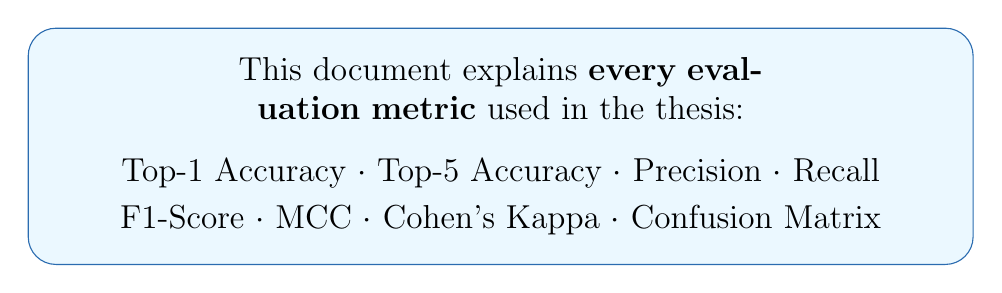
\begin{tikzpicture}
    \node[draw=medblue, fill=lightblue, rounded corners=10pt, minimum width=12cm, minimum height=3cm, text width=11cm, align=center, font=\large] {
        This document explains \textbf{every evaluation metric} used in the thesis:\\[0.3cm]
        Top-1 Accuracy $\cdot$ Top-5 Accuracy $\cdot$ Precision $\cdot$ Recall\\[0.1cm]
        F1-Score $\cdot$ MCC $\cdot$ Cohen's Kappa $\cdot$ Confusion Matrix
    };
\end{tikzpicture}

\vfill
{\large Thesis Reference Document}\\[0.3cm]
{\large\today}
\end{titlepage}

\tableofcontents
\newpage

% ══════════════════════════════════════════════════════════════
%              SECTION 0: PREREQUISITES
% ══════════════════════════════════════════════════════════════
\section{Before We Begin: The Four Fundamental Counts}

Before understanding any metric, you need to understand four basic concepts that \textbf{every metric is built from}. These come from the \textbf{confusion matrix}.

\subsection{The Binary Case (Two Classes)}

Imagine a simple scenario: a model must decide if a video shows ``\textbf{Vault}'' or ``\textbf{Not Vault}''.

\begin{keyidea}[The Four Outcomes]
When a model makes a prediction, exactly one of four things happens:

\begin{enumerate}[leftmargin=2cm, itemsep=0.5cm]
    \item[\textcolor{tp_green}{\textbf{TP}}] \textbf{True Positive:} The video \textit{is} Vault, and the model \textit{correctly says} ``Vault.''\\
    $\Rightarrow$ \textcolor{darkgreen}{The model got it right on a positive example.}

    \item[\textcolor{tn_blue}{\textbf{TN}}] \textbf{True Negative:} The video is \textit{not} Vault, and the model \textit{correctly says} ``Not Vault.''\\
    $\Rightarrow$ \textcolor{darkblue}{The model got it right on a negative example.}

    \item[\textcolor{fp_red}{\textbf{FP}}] \textbf{False Positive:} The video is \textit{not} Vault, but the model \textit{wrongly says} ``Vault.''\\
    $\Rightarrow$ \textcolor{darkred}{False alarm! The model cried wolf.}

    \item[\textcolor{fn_orange}{\textbf{FN}}] \textbf{False Negative:} The video \textit{is} Vault, but the model \textit{wrongly says} ``Not Vault.''\\
    $\Rightarrow$ \textcolor{darkorange}{The model missed a real case!}
\end{enumerate}
\end{keyidea}

\subsection{Visual Representation: The Confusion Matrix}

\begin{center}
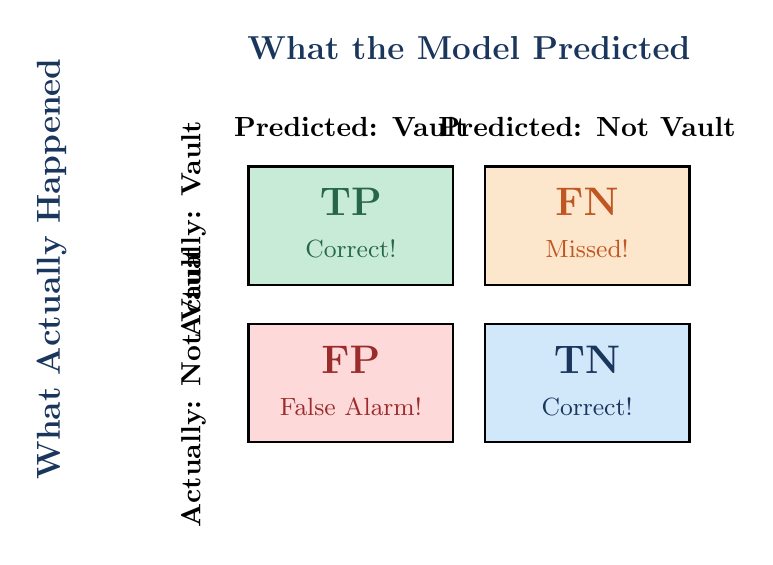
\begin{tikzpicture}[scale=1.0]
    % Headers
    \node[font=\large\bfseries, text=darkblue] at (3.5, 4.8) {What the Model Predicted};
    \node[font=\large\bfseries, text=darkblue, rotate=90] at (-1.8, 2) {What Actually Happened};

    \node[font=\bfseries] at (2, 3.8) {Predicted: Vault};
    \node[font=\bfseries] at (5, 3.8) {Predicted: Not Vault};
    \node[font=\bfseries, rotate=90] at (0, 2.5) {Actually: Vault};
    \node[font=\bfseries, rotate=90] at (0, 0.5) {Actually: Not Vault};

    % TP cell
    \fill[tp_green!30] (0.7, 1.8) rectangle (3.3, 3.3);
    \draw[thick] (0.7, 1.8) rectangle (3.3, 3.3);
    \node[font=\Large\bfseries, text=darkgreen] at (2, 2.85) {TP};
    \node[font=\small, text=darkgreen] at (2, 2.25) {Correct!};

    % FN cell
    \fill[fn_orange!30] (3.7, 1.8) rectangle (6.3, 3.3);
    \draw[thick] (3.7, 1.8) rectangle (6.3, 3.3);
    \node[font=\Large\bfseries, text=darkorange] at (5, 2.85) {FN};
    \node[font=\small, text=darkorange] at (5, 2.25) {Missed!};

    % FP cell
    \fill[fp_red!30] (0.7, -0.2) rectangle (3.3, 1.3);
    \draw[thick] (0.7, -0.2) rectangle (3.3, 1.3);
    \node[font=\Large\bfseries, text=darkred] at (2, 0.85) {FP};
    \node[font=\small, text=darkred] at (2, 0.25) {False Alarm!};

    % TN cell
    \fill[tn_blue!30] (3.7, -0.2) rectangle (6.3, 1.3);
    \draw[thick] (3.7, -0.2) rectangle (6.3, 1.3);
    \node[font=\Large\bfseries, text=darkblue] at (5, 0.85) {TN};
    \node[font=\small, text=darkblue] at (5, 0.25) {Correct!};
\end{tikzpicture}
\end{center}

\subsection{Multi-Class Extension}

In your thesis, you have \textbf{4 classes} (FineGym) or \textbf{51 classes} (HMDB51). For multi-class problems, we compute TP, FP, FN \textit{for each class separately} using a ``one-vs-rest'' approach:

\begin{examplebox}[FineGym Example: Computing TP / FP / FN for Balance Beam]
For the Balance Beam class specifically:
\begin{itemize}
    \item \textbf{TP} = Videos that ARE Balance Beam and model said ``Balance Beam''
    \item \textbf{FP} = Videos that are NOT Balance Beam but model wrongly said ``Balance Beam'' (maybe they were Floor Exercise)
    \item \textbf{FN} = Videos that ARE Balance Beam but model said something else (maybe ``Uneven Bars'')
\end{itemize}
Then we repeat this for Floor Exercise, Uneven Bars, and Vault.
\end{examplebox}


% ══════════════════════════════════════════════════════════════
%                   SECTION 1: TOP-1 ACCURACY
% ══════════════════════════════════════════════════════════════
\newpage
\section{Top-1 Accuracy}

\subsection{The Simple Question}

\begin{keyidea}[What Top-1 Accuracy Asks]
\textbf{``Is the model's single best guess correct?''}\\[0.3cm]
The model looks at a video and outputs probabilities for every class. We take the class with the \textbf{highest probability} (the model's ``best guess'') and check: does it match the true label?
\end{keyidea}

\subsection{The Formula}

\begin{formulabox}[Mathematical Definition]
\[
\boxed{\text{Top-1 Accuracy} = \frac{\text{Number of correctly classified samples}}{\text{Total number of samples}} = \frac{1}{N}\sum_{i=1}^{N} \mathbf{1}\big[\hat{y}_i = y_i\big]}
\]
where:
\begin{itemize}
    \item $N$ = total number of test samples
    \item $y_i$ = the true label of sample $i$ (ground truth)
    \item $\hat{y}_i = \arg\max_c \, p(c \mid \mathbf{x}_i)$ = the class with the highest predicted probability
    \item $\mathbf{1}[\cdot]$ = indicator function (equals 1 if the condition is true, 0 otherwise)
\end{itemize}
\end{formulabox}

\subsection{Worked Example}

\begin{examplebox}[Step-by-Step Example with 10 Videos]
Suppose we test on 10 FineGym videos. The model's top-1 prediction for each:

\begin{center}
\begin{tabular}{cllc}
\toprule
\textbf{Video} & \textbf{True Label} & \textbf{Model's Top-1 Prediction} & \textbf{Correct?} \\
\midrule
1 & Balance Beam & Balance Beam & \textcolor{darkgreen}{\checkmark} \\
2 & Floor Exercise & Floor Exercise & \textcolor{darkgreen}{\checkmark} \\
3 & Uneven Bars & Balance Beam & \textcolor{darkred}{\ding{55}} \\
4 & Vault & Vault & \textcolor{darkgreen}{\checkmark} \\
5 & Balance Beam & Balance Beam & \textcolor{darkgreen}{\checkmark} \\
6 & Floor Exercise & Vault & \textcolor{darkred}{\ding{55}} \\
7 & Uneven Bars & Uneven Bars & \textcolor{darkgreen}{\checkmark} \\
8 & Vault & Vault & \textcolor{darkgreen}{\checkmark} \\
9 & Balance Beam & Balance Beam & \textcolor{darkgreen}{\checkmark} \\
10 & Floor Exercise & Floor Exercise & \textcolor{darkgreen}{\checkmark} \\
\bottomrule
\end{tabular}
\end{center}

\[
\text{Top-1 Accuracy} = \frac{8 \text{ correct}}{10 \text{ total}} = 0.80 = 80\%
\]
\end{examplebox}



\subsection{Why Top-1 Accuracy Is Needed}

\begin{enumerate}[leftmargin=*, itemsep=0.3cm]
    \item \textbf{Most intuitive metric} --- everyone understands ``80\% of predictions were correct''
    \item \textbf{Universal benchmark} --- every paper in action recognition reports it, enabling direct comparison
    \item \textbf{Strictest test} --- the model must get its single best guess exactly right
\end{enumerate}

\subsection{The Dangerous Limitation of Accuracy}

\begin{warningbox}[Why Accuracy Alone Can Be Misleading]
\textbf{The Class Imbalance Problem:}\\[0.3cm]
Imagine a dataset with 950 ``walking'' videos and 50 ``falling'' videos (total = 1000).

A completely \textit{useless} model that \textbf{always predicts ``walking''} (ignoring the input entirely) would get:
\[
\text{Accuracy} = \frac{950}{1000} = 95\%
\]
That looks impressive! But the model \textbf{never detects a single fall}. It has completely failed at the important task.\\[0.3cm]
\textcolor{darkred}{\textbf{This is exactly why we need additional metrics like F1, MCC, and Kappa.}}
\end{warningbox}


% ══════════════════════════════════════════════════════════════
%                   SECTION 2: TOP-5 ACCURACY
% ══════════════════════════════════════════════════════════════
\newpage
\section{Top-5 Accuracy}

\subsection{The Softer Question}

\begin{keyidea}[What Top-5 Accuracy Asks]
\textbf{``Is the correct answer anywhere in the model's top 5 guesses?''}\\[0.3cm]
Instead of requiring the \#1 prediction to be correct, we check if the true label appears in the 5 most confident predictions. This gives the model some ``room for error.''
\end{keyidea}

\subsection{The Formula}

\begin{formulabox}[Mathematical Definition]
\[
\boxed{\text{Top-5 Accuracy} = \frac{1}{N}\sum_{i=1}^{N} \mathbf{1}\big[y_i \in \text{Top5}(\hat{\mathbf{p}}_i)\big]}
\]
where $\text{Top5}(\hat{\mathbf{p}}_i)$ returns the 5 classes with the highest predicted probabilities for sample $i$.
\end{formulabox}

\subsection{Worked Example}

\begin{examplebox}[Step-by-Step: One HMDB51 Video]
The model sees a video of someone \textbf{fencing} and outputs probabilities for all 51 classes. The top 5 are:

\begin{center}
\begin{tabular}{clc}
\toprule
\textbf{Rank} & \textbf{Predicted Class} & \textbf{Probability} \\
\midrule
1 & Sword Exercise & 0.25 \\
2 & Kick & 0.18 \\
\rowcolor{lightgreen} \textbf{3} & \textbf{Fencing} & \textbf{0.14} \\
4 & Punch & 0.12 \\
5 & Draw Sword & 0.09 \\
\midrule
6--51 & (other 46 classes) & (remaining 0.22) \\
\bottomrule
\end{tabular}
\end{center}

The true label is \textbf{Fencing}:
\begin{itemize}
    \item \textbf{Top-1:} \textcolor{darkred}{\ding{55} Incorrect} --- the \#1 prediction is ``Sword Exercise,'' not ``Fencing''
    \item \textbf{Top-5:} \textcolor{darkgreen}{\checkmark Correct} --- ``Fencing'' appears at rank \#3, which is within the top 5
\end{itemize}
\end{examplebox}

\subsection{Why Top-5 Accuracy Only for HMDB51, Not FineGym}

\begin{warningbox}[Important: Top-5 Is Meaningless for 4 Classes]
\textbf{FineGym has only 4 classes} (BB, FX, UB, VT).\\[0.3cm]
If you check whether the correct class is in the ``top 5'' of 4 classes, the answer is \textbf{always yes} --- because all 4 classes \textit{are} within the top 5. The metric would be 100\% for every model, telling you nothing.\\[0.3cm]
\textbf{HMDB51 has 51 classes}, so Top-5 is meaningful --- the correct class genuinely might not be in the top 5 guesses.
\end{warningbox}

\subsection{What the Top-1 vs Top-5 Gap Tells You}

\begin{intuitionbox}[Reading the Gap Between Top-1 and Top-5]
The difference between Top-1 and Top-5 accuracy reveals \textbf{how confused the model is between similar classes}.

\begin{center}
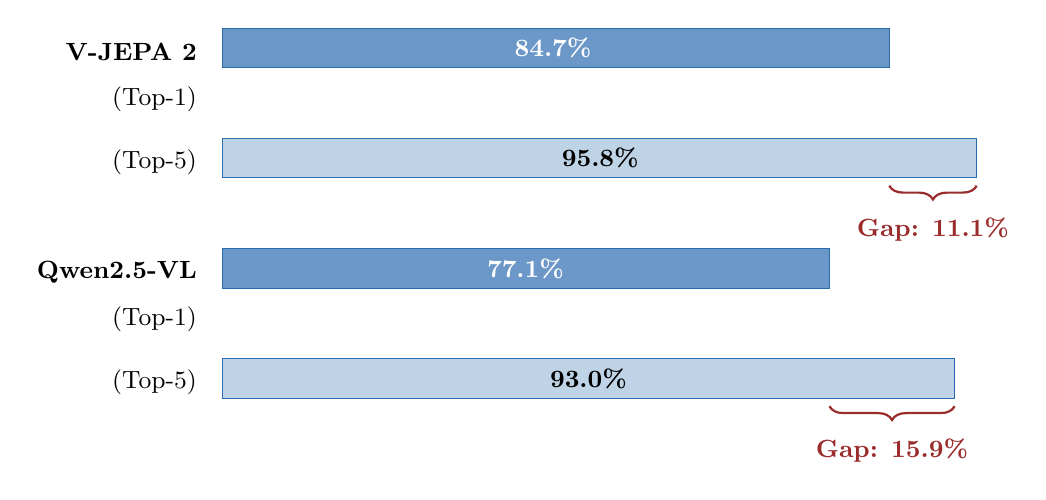
\begin{tikzpicture}[
    bar/.style={fill=medblue!70, draw=medblue, minimum height=0.6cm, anchor=west},
    bar5/.style={fill=medblue!30, draw=medblue, minimum height=0.6cm, anchor=west},
    label/.style={anchor=east, font=\small\bfseries}
]
    % V-JEPA 2
    \node[label] at (-0.2, 2.2) {V-JEPA 2};
    \node[label, font=\small] at (-0.2, 1.6) {(Top-1)};
    \draw[bar, minimum width=8.47cm] (0, 2) rectangle +(8.47, 0.5);
    \node[font=\small\bfseries, white] at (4.2, 2.25) {84.7\%};

    \node[label, font=\small] at (-0.2, 0.8) {(Top-5)};
    \draw[bar5, minimum width=9.58cm] (0, 0.6) rectangle +(9.58, 0.5);
    \node[font=\small\bfseries] at (4.8, 0.85) {95.8\%};

    \draw[decorate, decoration={brace, amplitude=5pt, mirror}, thick, darkred]
        (8.47, 0.5) -- (9.58, 0.5) node[midway, below=8pt, font=\small\bfseries, text=darkred] {Gap: 11.1\%};

    % Qwen
    \node[label] at (-0.2, -0.6) {Qwen2.5-VL};
    \node[label, font=\small] at (-0.2, -1.2) {(Top-1)};
    \draw[bar, minimum width=7.71cm] (0, -0.8) rectangle +(7.71, 0.5);
    \node[font=\small\bfseries, white] at (3.85, -0.55) {77.1\%};

    \node[label, font=\small] at (-0.2, -2.0) {(Top-5)};
    \draw[bar5, minimum width=9.30cm] (0, -2.2) rectangle +(9.30, 0.5);
    \node[font=\small\bfseries] at (4.65, -1.95) {93.0\%};

    \draw[decorate, decoration={brace, amplitude=5pt, mirror}, thick, darkred]
        (7.71, -2.3) -- (9.30, -2.3) node[midway, below=8pt, font=\small\bfseries, text=darkred] {Gap: 15.9\%};
\end{tikzpicture}
\end{center}

\textbf{Interpretation:}
\begin{itemize}
    \item \textbf{V-JEPA 2} (gap = 11.1\%): The model is fairly confident. When it's wrong, the correct answer is usually its \#2 or \#3 guess.
    \item \textbf{Qwen2.5-VL} (gap = 15.9\%): More confusion between similar classes. It knows the ``neighborhood'' but struggles with the exact class more often.
\end{itemize}

\textbf{Smaller gap = more precise model. Larger gap = model is confused between similar classes.}
\end{intuitionbox}


% ══════════════════════════════════════════════════════════════
%                   SECTION 3: PRECISION
% ══════════════════════════════════════════════════════════════
\newpage
\section{Precision}

\subsection{The Core Question}

\begin{keyidea}[What Precision Asks]
\textbf{``When the model says `this is class X,' how often is it actually correct?''}\\[0.3cm]
Precision measures \textbf{how trustworthy} the model's predictions are. High precision means: when the model says ``Vault,'' you can trust that it really is Vault.
\end{keyidea}

\subsection{The Formula}

\begin{formulabox}[Mathematical Definition]
For a single class $c$:
\[
\boxed{\text{Precision}_c = \frac{TP_c}{TP_c + FP_c}}
\]
In words:
\[
\text{Precision} = \frac{\text{Correctly predicted as class } c}{\text{Everything the model predicted as class } c}
\]
\end{formulabox}

\subsection{Worked Example}

\begin{examplebox}[FineGym: Precision for ``Balance Beam'']
Suppose out of 55 test videos total:
\begin{itemize}
    \item The model predicted 18 videos as ``Balance Beam''
    \item Of those 18 predictions, \textbf{15 were actually Balance Beam} (TP = 15)
    \item But \textbf{3 were actually Uneven Bars} that the model got wrong (FP = 3)
\end{itemize}

\[
\text{Precision}_{\text{BB}} = \frac{15}{15 + 3} = \frac{15}{18} = 0.833 = 83.3\%
\]

\textbf{Meaning:} When the model says ``Balance Beam,'' it's right 83.3\% of the time.
\end{examplebox}

\subsection{Macro vs.\ Weighted Precision}

Since we have multiple classes, we need to combine per-class precisions into a single number.

\begin{center}
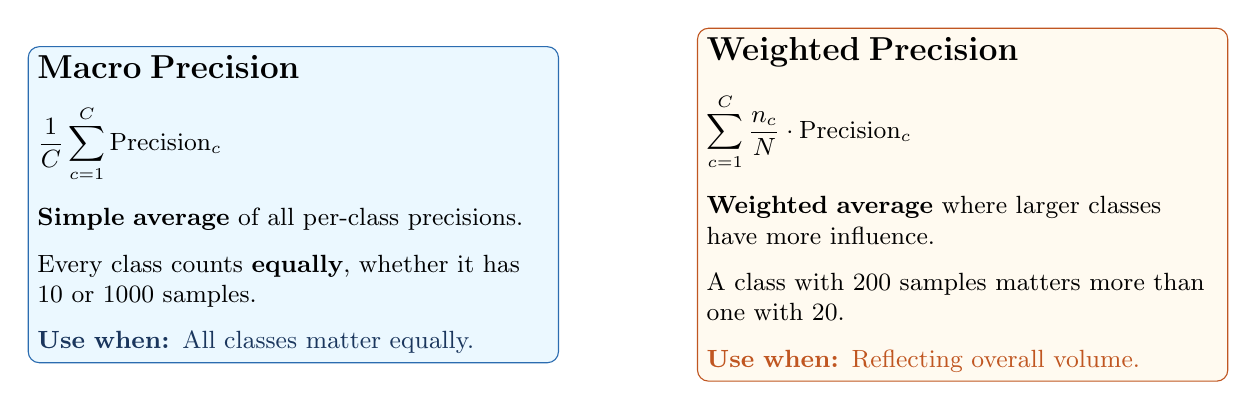
\begin{tikzpicture}
    % Macro box
    \node[draw=medblue, fill=lightblue, rounded corners, text width=6.5cm, minimum height=4cm, align=left, font=\small] (macro) at (0, 0) {
        \textbf{\large Macro Precision}\\[0.3cm]
        $\displaystyle\frac{1}{C}\sum_{c=1}^{C} \text{Precision}_c$\\[0.3cm]
        \textbf{Simple average} of all per-class precisions.\\[0.2cm]
        Every class counts \textbf{equally}, whether it has 10 or 1000 samples.\\[0.2cm]
        \textcolor{darkblue}{\textbf{Use when:} All classes matter equally.}
    };

    % Weighted box
    \node[draw=darkorange, fill=lightorange, rounded corners, text width=6.5cm, minimum height=4cm, align=left, font=\small] (weighted) at (8.5, 0) {
        \textbf{\large Weighted Precision}\\[0.3cm]
        $\displaystyle\sum_{c=1}^{C} \frac{n_c}{N} \cdot \text{Precision}_c$\\[0.3cm]
        \textbf{Weighted average} where larger classes have more influence.\\[0.2cm]
        A class with 200 samples matters more than one with 20.\\[0.2cm]
        \textcolor{darkorange}{\textbf{Use when:} Reflecting overall volume.}
    };
\end{tikzpicture}
\end{center}

\begin{examplebox}[Macro vs Weighted --- Numerical Example]
Suppose 3 classes with different numbers of test samples:

\begin{center}
\begin{tabular}{lccc}
\toprule
\textbf{Class} & \textbf{Precision} & \textbf{Test Samples} & \textbf{Weight ($n_c/N$)} \\
\midrule
Balance Beam & 90\% & 100 & 100/200 = 0.50 \\
Floor Exercise & 80\% & 80 & 80/200 = 0.40 \\
Vault & 60\% & 20 & 20/200 = 0.10 \\
\midrule
\textbf{Total} & & 200 & 1.00 \\
\bottomrule
\end{tabular}
\end{center}

\textbf{Macro Precision} = $\frac{90 + 80 + 60}{3}$ = \textbf{76.7\%}\\[0.2cm]
\textbf{Weighted Precision} = $0.50 \times 90 + 0.40 \times 80 + 0.10 \times 60$ = $45 + 32 + 6$ = \textbf{83.0\%}\\[0.3cm]
Weighted is higher because the model does best on Balance Beam, which has the most samples.
\end{examplebox}


% ══════════════════════════════════════════════════════════════
%                   SECTION 4: RECALL
% ══════════════════════════════════════════════════════════════
\newpage
\section{Recall (Sensitivity)}

\subsection{The Core Question}

\begin{keyidea}[What Recall Asks]
\textbf{``Of all the videos that actually ARE class X, how many did the model successfully find?''}\\[0.3cm]
Recall measures \textbf{how completely} the model detects all instances of a class. High recall means: the model rarely \textit{misses} a real instance.
\end{keyidea}

\subsection{The Formula}

\begin{formulabox}[Mathematical Definition]
For a single class $c$:
\[
\boxed{\text{Recall}_c = \frac{TP_c}{TP_c + FN_c}}
\]
In words:
\[
\text{Recall} = \frac{\text{Correctly identified instances of class } c}{\text{All actual instances of class } c}
\]
\end{formulabox}

\subsection{Worked Example}

\begin{examplebox}[FineGym: Recall for ``Balance Beam'']
Suppose there are \textbf{20 actual Balance Beam videos} in the test set:
\begin{itemize}
    \item The model correctly identified \textbf{15 of them} as Balance Beam (TP = 15)
    \item But it \textbf{missed 5} --- it wrongly called them Uneven Bars or Floor Exercise (FN = 5)
\end{itemize}

\[
\text{Recall}_{\text{BB}} = \frac{15}{15 + 5} = \frac{15}{20} = 0.75 = 75\%
\]

\textbf{Meaning:} The model found 75\% of all actual Balance Beam videos. It missed 25\%.
\end{examplebox}

\subsection{Precision vs.\ Recall: The Fundamental Tradeoff}

These two metrics are \textbf{inherently in tension}:

\begin{center}
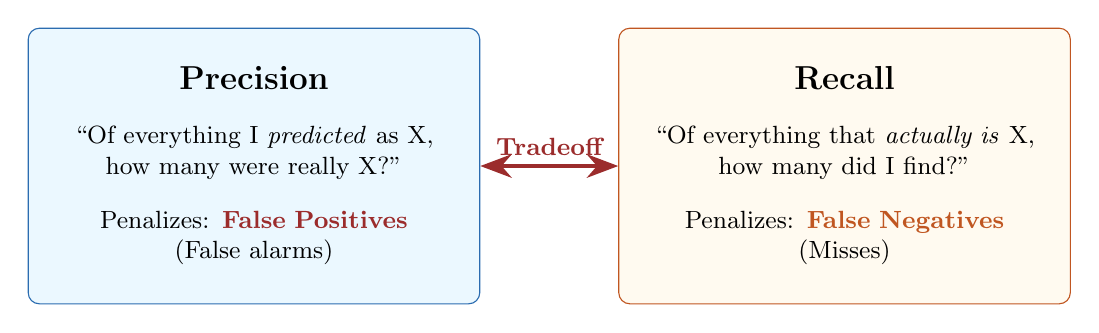
\begin{tikzpicture}[
    box/.style={draw, rounded corners, text width=5.5cm, minimum height=3.5cm, align=center, font=\small}
]
    \node[box, fill=lightblue, draw=medblue] (prec) at (0, 0) {
        \textbf{\large Precision}\\[0.3cm]
        ``Of everything I \textit{predicted} as X,\\how many were really X?''\\[0.3cm]
        Penalizes: \textcolor{darkred}{\textbf{False Positives}}\\(False alarms)
    };

    \node[box, fill=lightorange, draw=darkorange] (rec) at (7.5, 0) {
        \textbf{\large Recall}\\[0.3cm]
        ``Of everything that \textit{actually is} X,\\how many did I find?''\\[0.3cm]
        Penalizes: \textcolor{darkorange}{\textbf{False Negatives}}\\(Misses)
    };

    \draw[{Stealth[length=4mm]}-{Stealth[length=4mm]}, very thick, darkred] (prec.east) -- (rec.west)
        node[midway, above, font=\small\bfseries] {Tradeoff};
\end{tikzpicture}
\end{center}

\begin{intuitionbox}[Real-World Analogy]
Think of a \textbf{security guard} checking IDs at a gate:

\begin{itemize}[itemsep=0.3cm]
    \item \textbf{High Precision, Low Recall:} The guard is very strict --- only lets people through when absolutely certain. Almost never lets in an intruder (low FP), but frequently turns away legitimate visitors (high FN).
    \item \textbf{High Recall, Low Precision:} The guard lets almost everyone in to make sure no legitimate visitor is rejected. Catches all legitimate visitors (low FN), but also lets in some intruders (high FP).
    \item \textbf{High Both:} A perfect guard who correctly identifies almost everyone.
\end{itemize}
\end{intuitionbox}


% ══════════════════════════════════════════════════════════════
%                   SECTION 5: F1-SCORE
% ══════════════════════════════════════════════════════════════
\newpage
\section{F1-Score}

\subsection{Why We Need F1}

Since precision and recall are in tension, we want a \textbf{single number} that balances both. That's the F1-Score.

\begin{keyidea}[What F1-Score Is]
\textbf{The harmonic mean of Precision and Recall.}\\[0.3cm]
It gives a single number that is high \textbf{only when BOTH precision and recall are high}. If either one is low, F1 drops dramatically.
\end{keyidea}

\subsection{The Formula}

\begin{formulabox}[Mathematical Definition]
\[
\boxed{F1_c = 2 \times \frac{\text{Precision}_c \times \text{Recall}_c}{\text{Precision}_c + \text{Recall}_c} = \frac{2 \cdot TP_c}{2 \cdot TP_c + FP_c + FN_c}}
\]
\end{formulabox}

\subsection{Why Harmonic Mean, Not Regular Average?}

This is a critical point. The harmonic mean \textbf{punishes imbalance} much more harshly:

\begin{center}
\begin{tabular}{cccc}
\toprule
\textbf{Precision} & \textbf{Recall} & \textbf{Regular Average} & \textbf{Harmonic Mean (F1)} \\
\midrule
100\% & 0\% & 50\% & \textcolor{darkred}{\textbf{0\%}} \\
90\% & 10\% & 50\% & \textcolor{darkred}{\textbf{18\%}} \\
80\% & 40\% & 60\% & \textcolor{darkorange}{\textbf{53\%}} \\
80\% & 80\% & 80\% & \textcolor{darkgreen}{\textbf{80\%}} \\
95\% & 90\% & 92.5\% & \textcolor{darkgreen}{\textbf{92.4\%}} \\
\bottomrule
\end{tabular}
\end{center}

\begin{intuitionbox}[Why This Matters]
A model that has 100\% precision but 0\% recall (it never predicts any class, so it's never wrong but also never finds anything) would get 50\% on a regular average --- which sounds decent. But F1 correctly gives it \textbf{0\%}, reflecting that the model is useless.
\end{intuitionbox}

\subsection{Worked Example}

\begin{examplebox}[Complete F1 Calculation for ``Balance Beam'']
From our earlier examples:
\begin{itemize}
    \item Precision$_{\text{BB}}$ = 83.3\% (15 correct out of 18 predictions)
    \item Recall$_{\text{BB}}$ = 75.0\% (15 found out of 20 actual)
\end{itemize}

\[
F1_{\text{BB}} = 2 \times \frac{0.833 \times 0.750}{0.833 + 0.750} = 2 \times \frac{0.625}{1.583} = 2 \times 0.395 = \textbf{0.789 = 78.9\%}
\]
\end{examplebox}

\subsection{Macro F1 vs.\ Weighted F1}

\begin{center}
\begin{tabular}{lll}
\toprule
\textbf{Variant} & \textbf{Formula} & \textbf{Used For} \\
\midrule
\textbf{Macro F1} & $\frac{1}{C}\sum_{c=1}^{C} F1_c$ & Model selection in your code \\
\textbf{Weighted F1} & $\sum_{c=1}^{C} \frac{n_c}{N} F1_c$ & Overall performance summary \\
\bottomrule
\end{tabular}
\end{center}

\begin{keyidea}[F1 Is Your Primary Model Selection Metric]
In your code, the best classifier is chosen by \textbf{Macro F1}, not accuracy:
\begin{center}
\texttt{if f1 > best\_f1: best\_f1 = f1; best\_name = cname}
\end{center}
This is the correct choice because Macro F1 is robust to class imbalance and ensures rare classes are not ignored.
\end{keyidea}


% ══════════════════════════════════════════════════════════════
%                   SECTION 6: MCC
% ══════════════════════════════════════════════════════════════
\newpage
\section{Matthews Correlation Coefficient (MCC)}

\subsection{The Most Balanced Metric}

\begin{keyidea}[What MCC Is]
MCC is a \textbf{correlation coefficient} between the model's predictions and the actual ground truth. It is widely regarded as the \textbf{single most informative and balanced metric} for classification.\\[0.3cm]
It is the \textbf{only metric that uses all four cells} of the confusion matrix (TP, TN, FP, FN) symmetrically.
\end{keyidea}

\subsection{The Formula}

\begin{formulabox}[Mathematical Definition (Binary Case)]
\[
\boxed{MCC = \frac{TP \times TN - FP \times FN}{\sqrt{(TP+FP)(TP+FN)(TN+FP)(TN+FN)}}}
\]
For multi-class (what scikit-learn computes), it generalizes using the full confusion matrix $\mathbf{C}$:
\[
MCC = \frac{c \cdot s - \sum_k p_k \cdot t_k}{\sqrt{(s^2 - \sum_k p_k^2)(s^2 - \sum_k t_k^2)}}
\]
where $c$ = total correct predictions, $s$ = total samples, $p_k$ = times class $k$ was predicted, $t_k$ = true occurrences of class $k$.
\end{formulabox}

\subsection{Value Range and Interpretation}

\begin{center}
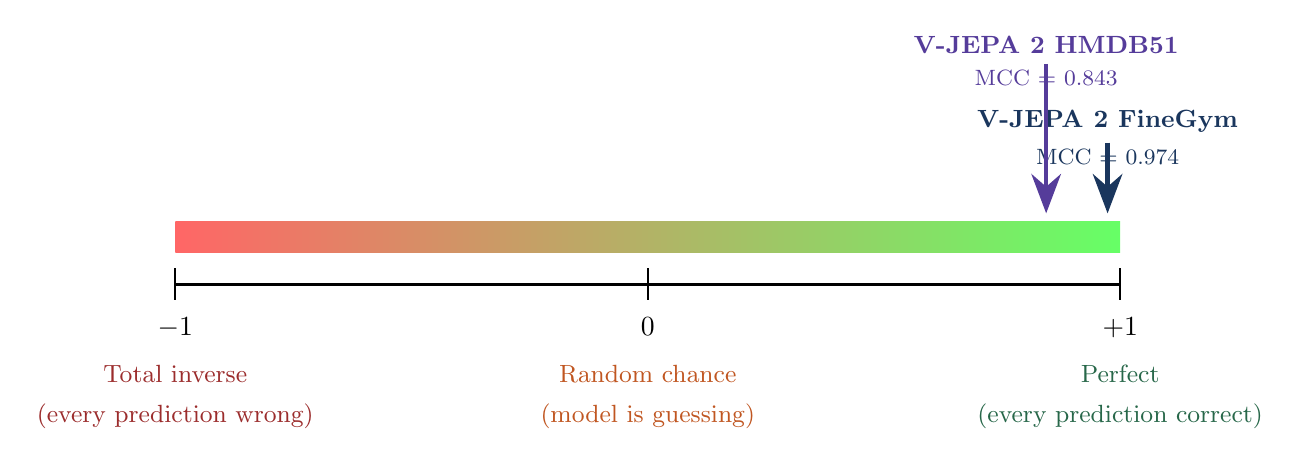
\begin{tikzpicture}[scale=1.0]
    % Scale bar
    \draw[very thick] (0, 0) -- (12, 0);

    % Tick marks and labels
    \draw[thick] (0, -0.2) -- (0, 0.2);
    \node[below, font=\bfseries] at (0, -0.3) {$-1$};
    \node[below, font=\small, text=darkred] at (0, -0.9) {Total inverse};
    \node[below, font=\small, text=darkred] at (0, -1.4) {(every prediction wrong)};

    \draw[thick] (6, -0.2) -- (6, 0.2);
    \node[below, font=\bfseries] at (6, -0.3) {$0$};
    \node[below, font=\small, text=darkorange] at (6, -0.9) {Random chance};
    \node[below, font=\small, text=darkorange] at (6, -1.4) {(model is guessing)};

    \draw[thick] (12, -0.2) -- (12, 0.2);
    \node[below, font=\bfseries] at (12, -0.3) {$+1$};
    \node[below, font=\small, text=darkgreen] at (12, -0.9) {Perfect};
    \node[below, font=\small, text=darkgreen] at (12, -1.4) {(every prediction correct)};

    % Color gradient
    \shade[left color=red!60, right color=green!60] (0, 0.4) rectangle (12, 0.8);

    % Your results
    \draw[ultra thick, darkblue, -{Stealth[length=5mm]}] (11.84, 1.8) -- (11.84, 0.9);
    \node[above, font=\small\bfseries, text=darkblue] at (11.84, 1.8) {V-JEPA 2 FineGym};
    \node[above, font=\footnotesize, text=darkblue] at (11.84, 1.4) {MCC = 0.974};

    \draw[ultra thick, darkpurple, -{Stealth[length=5mm]}] (11.06, 2.8) -- (11.06, 0.9);
    \node[above, font=\small\bfseries, text=darkpurple] at (11.06, 2.8) {V-JEPA 2 HMDB51};
    \node[above, font=\footnotesize, text=darkpurple] at (11.06, 2.4) {MCC = 0.843};
\end{tikzpicture}
\end{center}

\subsection{Why MCC Is Special --- The ``Accuracy Trap'' Example}

\begin{warningbox}[MCC Catches What Accuracy Misses]
\textbf{Scenario:} 950 test samples are class A, 50 are class B.\\
\textbf{Useless model:} Always predicts class A (ignores input completely).

\begin{center}
\begin{tabular}{lcc}
\toprule
& \textbf{Accuracy} & \textbf{MCC} \\
\midrule
Useless model (always A) & \textcolor{darkred}{95.0\%} $\leftarrow$ looks great! & \textcolor{darkgreen}{0.000} $\leftarrow$ correctly says ``random'' \\
\midrule
Good model & 92.0\% & 0.750 \\
\bottomrule
\end{tabular}
\end{center}

Accuracy would \textbf{wrongly} rank the useless model higher! MCC correctly identifies it as no better than chance.
\end{warningbox}

\begin{examplebox}[MCC Worked Example (Binary)]
$TP = 40,\; TN = 45,\; FP = 5,\; FN = 10$

\[
MCC = \frac{40 \times 45 - 5 \times 10}{\sqrt{(40+5)(40+10)(45+5)(45+10)}}
= \frac{1800 - 50}{\sqrt{45 \times 50 \times 50 \times 55}}
= \frac{1750}{\sqrt{6{,}187{,}500}}
= \frac{1750}{2487.5}
= \textbf{0.703}
\]
Interpretation: Strong positive correlation --- the model's predictions align well with truth.
\end{examplebox}


% ══════════════════════════════════════════════════════════════
%                   SECTION 7: COHEN'S KAPPA
% ══════════════════════════════════════════════════════════════
\newpage
\section{Cohen's Kappa ($\kappa$)}

\subsection{The Core Question}

\begin{keyidea}[What Cohen's Kappa Asks]
\textbf{``How much better is the model than pure random chance?''}\\[0.3cm]
Kappa adjusts accuracy by subtracting out the agreement that would happen purely by luck. A model that gets 90\% accuracy on an easy problem (where random guessing gets 80\%) is not as impressive as one that gets 80\% on a hard problem (where random guessing gets 2\%).
\end{keyidea}

\subsection{The Formula}

\begin{formulabox}[Mathematical Definition]
\[
\boxed{\kappa = \frac{p_o - p_e}{1 - p_e}}
\]
where:
\begin{itemize}
    \item $p_o$ = \textbf{observed agreement} = accuracy = fraction of correct predictions
    \item $p_e$ = \textbf{expected agreement by chance} = probability that a random model would be correct, given the class distribution
\end{itemize}

For multi-class:
\[
p_e = \sum_{c=1}^{C} \frac{n_{c,\text{pred}} \times n_{c,\text{true}}}{N^2}
\]
where $n_{c,\text{pred}}$ = how many times the model predicted class $c$, and $n_{c,\text{true}}$ = how many times class $c$ actually appeared.
\end{formulabox}

\subsection{Worked Example}

\begin{examplebox}[Cohen's Kappa Step-by-Step]
\textbf{Given:} 100 test samples, 2 classes (A and B). The confusion matrix is:

\begin{center}
\begin{tabular}{lcc|c}
\toprule
& \textbf{Predicted A} & \textbf{Predicted B} & \textbf{Total (True)} \\
\midrule
\textbf{True A} & 40 & 10 & 50 \\
\textbf{True B} & 5 & 45 & 50 \\
\midrule
\textbf{Total (Pred)} & 45 & 55 & 100 \\
\bottomrule
\end{tabular}
\end{center}

\textbf{Step 1:} Observed agreement:
$p_o = \frac{40 + 45}{100} = 0.85$

\textbf{Step 2:} Expected agreement by chance:
\[
p_e = \frac{45 \times 50}{100^2} + \frac{55 \times 50}{100^2} = \frac{2250}{10000} + \frac{2750}{10000} = 0.225 + 0.275 = 0.50
\]
(A random model would get 50\% right just by the distribution of predictions and labels.)

\textbf{Step 3:} Kappa:
\[
\kappa = \frac{0.85 - 0.50}{1 - 0.50} = \frac{0.35}{0.50} = \textbf{0.70}
\]
\end{examplebox}

\subsection{Standard Interpretation Scale}

\begin{center}
\begin{tabular}{lll}
\toprule
\textbf{$\kappa$ Range} & \textbf{Agreement Level} & \textbf{Your Results} \\
\midrule
$< 0.00$ & Less than chance & \\
$0.01 - 0.20$ & Slight & \\
$0.21 - 0.40$ & Fair & \\
$0.41 - 0.60$ & Moderate & \\
$0.61 - 0.80$ & Substantial & Qwen HMDB51 ($\kappa = 0.765$) \\
\rowcolor{lightgreen}
$0.81 - 1.00$ & \textbf{Almost Perfect} & \textbf{V-JEPA 2: 0.974 (FG), 0.842 (HM)} \\
\bottomrule
\end{tabular}
\end{center}

\subsection{Kappa vs.\ MCC: What's the Difference?}

\begin{center}
\begin{tabular}{lll}
\toprule
& \textbf{MCC} & \textbf{Cohen's Kappa ($\kappa$)} \\
\midrule
\textbf{Origin} & Statistics (Pearson's $\phi$) & Psychology (inter-rater reliability) \\
\textbf{Measures} & Correlation between predictions \& truth & Improvement over random chance \\
\textbf{Range} & $[-1, +1]$ & $[-1, +1]$ (typically $[0, 1]$) \\
\textbf{In practice} & Often $\approx \kappa$ & Often $\approx$ MCC \\
\bottomrule
\end{tabular}
\end{center}

In your results, MCC and $\kappa$ are nearly identical (e.g., both 0.974 on FineGym, both $\approx 0.843$ on HMDB51). Reporting \textbf{both} gives independent confirmation from two different statistical traditions.


% ══════════════════════════════════════════════════════════════
%                   SECTION 8: CONFUSION MATRIX
% ══════════════════════════════════════════════════════════════
\newpage
\section{The Confusion Matrix (Foundation of All Metrics)}

\subsection{What It Is}

\begin{keyidea}[The Confusion Matrix]
A $C \times C$ table (where $C$ = number of classes) that shows \textbf{exactly how many samples of each true class were predicted as each class}.\\[0.3cm]
Row $i$, Column $j$ = number of samples whose true label is $i$ but were predicted as $j$.
\end{keyidea}

\subsection{Visual Example: FineGym (Near-Perfect Model)}

\begin{center}
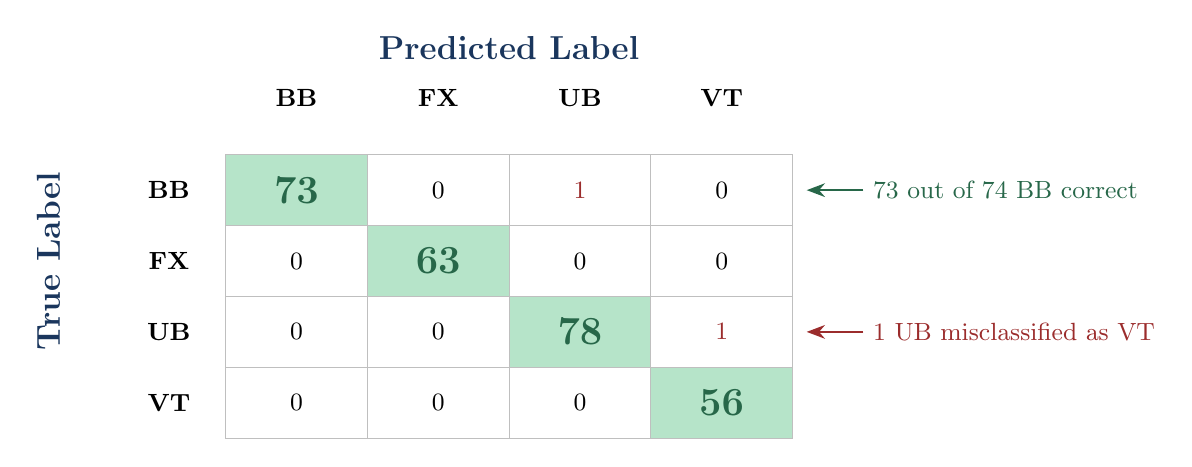
\begin{tikzpicture}[scale=0.9]
    \node[font=\large\bfseries, text=darkblue] at (4.5, 5.5) {Predicted Label};
    \node[font=\large\bfseries, text=darkblue, rotate=90] at (-2.0, 2.5) {True Label};

    % Column headers
    \node[font=\small\bfseries] at (1.5, 4.8) {BB};
    \node[font=\small\bfseries] at (3.5, 4.8) {FX};
    \node[font=\small\bfseries] at (5.5, 4.8) {UB};
    \node[font=\small\bfseries] at (7.5, 4.8) {VT};

    % Row headers
    \node[font=\small\bfseries] at (-0.3, 3.5) {BB};
    \node[font=\small\bfseries] at (-0.3, 2.5) {FX};
    \node[font=\small\bfseries] at (-0.3, 1.5) {UB};
    \node[font=\small\bfseries] at (-0.3, 0.5) {VT};

    % Diagonal (correct) - green
    \fill[tp_green!40] (0.5, 3) rectangle (2.5, 4);
    \fill[tp_green!40] (2.5, 2) rectangle (4.5, 3);
    \fill[tp_green!40] (4.5, 1) rectangle (6.5, 2);
    \fill[tp_green!40] (6.5, 0) rectangle (8.5, 1);

    % Off-diagonal (errors) - light red
    \foreach \x in {0.5, 2.5, 4.5, 6.5} {
        \foreach \y in {0, 1, 2, 3} {
            \draw[gray!50] (\x, \y) rectangle ++(2, 1);
        }
    }

    % Values
    \node[font=\Large\bfseries, text=darkgreen] at (1.5, 3.5) {73};
    \node[font=\small] at (3.5, 3.5) {0};
    \node[font=\small, text=darkred] at (5.5, 3.5) {1};
    \node[font=\small] at (7.5, 3.5) {0};

    \node[font=\small] at (1.5, 2.5) {0};
    \node[font=\Large\bfseries, text=darkgreen] at (3.5, 2.5) {63};
    \node[font=\small] at (5.5, 2.5) {0};
    \node[font=\small] at (7.5, 2.5) {0};

    \node[font=\small] at (1.5, 1.5) {0};
    \node[font=\small] at (3.5, 1.5) {0};
    \node[font=\Large\bfseries, text=darkgreen] at (5.5, 1.5) {78};
    \node[font=\small, text=darkred] at (7.5, 1.5) {1};

    \node[font=\small] at (1.5, 0.5) {0};
    \node[font=\small] at (3.5, 0.5) {0};
    \node[font=\small] at (5.5, 0.5) {0};
    \node[font=\Large\bfseries, text=darkgreen] at (7.5, 0.5) {56};

    % Annotations
    \draw[thick, darkgreen, -{Stealth}] (9.5, 3.5) -- (8.7, 3.5);
    \node[right, font=\small, text=darkgreen] at (9.5, 3.5) {73 out of 74 BB correct};

    \draw[thick, darkred, -{Stealth}] (9.5, 1.5) -- (8.7, 1.5);
    \node[right, font=\small, text=darkred] at (9.5, 1.5) {1 UB misclassified as VT};
\end{tikzpicture}
\end{center}

\subsection{How to Read the Confusion Matrix}

\begin{enumerate}[leftmargin=*, itemsep=0.3cm]
    \item \textbf{Diagonal cells} (green) = \textbf{correct predictions}. Larger numbers = better.
    \item \textbf{Off-diagonal cells} (errors) show \textit{which classes get confused with which}. For example, if cell (UB, BB) = 5, it means 5 Uneven Bars videos were wrongly classified as Balance Beam.
    \item \textbf{Row sums} = total actual samples per class.
    \item \textbf{Column sums} = total predictions per class.
\end{enumerate}

\begin{intuitionbox}[What the Confusion Matrix Reveals That No Single Number Can]
The confusion matrix answers questions like:
\begin{itemize}
    \item ``Which two classes does the model confuse most often?'' (look for large off-diagonal values)
    \item ``Is there one class the model almost never gets right?'' (look for a row with small diagonal value)
    \item ``Does the model over-predict a particular class?'' (column sum much larger than row sum)
\end{itemize}
\textbf{No single metric (accuracy, F1, MCC, etc.) can tell you WHERE the errors are --- only the confusion matrix can.}
\end{intuitionbox}


% ══════════════════════════════════════════════════════════════
%                   SECTION 9: WHY ALL METRICS TOGETHER
% ══════════════════════════════════════════════════════════════
\newpage
\section{Why We Need ALL These Metrics Together}

No single metric tells the complete story. Each one catches different failure modes.

\subsection{What Each Metric Catches That Others Miss}

\begin{center}
\renewcommand{\arraystretch}{1.3}
\begin{tabular}{>{\bfseries}p{2.8cm}p{5cm}p{5cm}}
\toprule
\textbf{Metric} & \textbf{What It Reveals} & \textbf{What It Misses} \\
\midrule
Top-1 Accuracy & How often the best guess is correct & Whether rare classes are ignored; whether the model is ``close'' when wrong \\
Top-5 Accuracy & Whether the model ``understands'' the problem even when wrong & Doesn't distinguish \#2 from \#5; inapplicable for few classes \\
Precision & How trustworthy positive predictions are & Whether the model finds all instances (recall) \\
Recall & How completely the model finds each class & Whether the ``found'' predictions are correct (precision) \\
F1-Score & Balance of precision and recall & Doesn't account for true negatives; can be gamed \\
MCC & Overall correlation using ALL confusion matrix cells & Doesn't show class-specific problems \\
Cohen's $\kappa$ & Improvement over random chance & Similar to MCC; adds interpretive scale \\
\bottomrule
\end{tabular}
\end{center}

\subsection{The Story They Tell Together}

Using your V-JEPA~2 HAF-STD Net results on HMDB51 as an example:

\begin{summarybox}[Complete Metric Story: V-JEPA~2 on HMDB51]
\begin{center}
\renewcommand{\arraystretch}{1.4}
\begin{tabular}{lrl}
\toprule
\textbf{Metric} & \textbf{Value} & \textbf{What This Tells Us} \\
\midrule
Top-1 Accuracy & 84.7\% & The model gets the exact right answer 85\% of the time \\
Top-5 Accuracy & 95.8\% & When wrong, the right answer is usually in the top 5 \\
Precision (macro) & 87.7\% & When it makes a prediction, it's usually correct \\
Recall (macro) & 84.8\% & It finds most instances of each action class \\
F1 (macro) & 85.3\% & Precision and recall are well-balanced \\
MCC & 0.843 & Strong genuine correlation, not a class-imbalance artifact \\
Cohen's $\kappa$ & 0.842 & Almost perfect agreement, far better than chance \\
\bottomrule
\end{tabular}
\end{center}

\textbf{Combined narrative:} The model is highly accurate (84.7\%), and even when it's wrong, it's usually ``close'' (95.8\% top-5). Its predictions are trustworthy (87.7\% precision) and comprehensive (84.8\% recall), with good balance between the two (85.3\% F1). This performance is genuine, not an artifact of class distribution (MCC = 0.843), and represents almost perfect agreement beyond chance ($\kappa$ = 0.842).
\end{summarybox}

\subsection{Danger of Using Only One Metric}

\begin{warningbox}[What Goes Wrong With Single Metrics]
\begin{center}
\renewcommand{\arraystretch}{1.3}
\begin{tabular}{p{4cm}p{9cm}}
\toprule
\textbf{If you only report\ldots} & \textbf{A reviewer could ask\ldots} \\
\midrule
Accuracy alone & ``Is this inflated by class imbalance? What about minority classes?'' \\
F1 alone & ``Is the model confident? How does it rank against chance?'' \\
Top-1 alone & ``Does the model completely fail when wrong, or is it close?'' \\
MCC alone & ``What's the actual accuracy? Which specific classes fail?'' \\
\bottomrule
\end{tabular}
\end{center}

\textbf{Reporting all seven metrics preemptively answers every possible reviewer question} about your model's classification quality.
\end{warningbox}


% ══════════════════════════════════════════════════════════════
%                   SECTION 10: QUICK REFERENCE
% ══════════════════════════════════════════════════════════════
\newpage
\section{Quick Reference Card}

\begin{summarybox}[All Metrics at a Glance]
\begin{center}
\renewcommand{\arraystretch}{1.5}
\begin{tabular}{p{2.8cm}ccccc}
\toprule
\textbf{Metric} & \textbf{Range} & \textbf{Perfect} & \textbf{Random} & \multicolumn{2}{c}{\textbf{Your Best (V-JEPA 2)}} \\
& & & & \textbf{FineGym} & \textbf{HMDB51} \\
\midrule
Top-1 Accuracy & $[0, 1]$ & 1.0 & $1/C$ & 98.1\% & 84.7\% \\
Top-5 Accuracy & $[0, 1]$ & 1.0 & $5/C$ & N/A & 95.8\% \\
Precision (macro) & $[0, 1]$ & 1.0 & $\sim 1/C$ & 98.5\% & 87.7\% \\
Recall (macro) & $[0, 1]$ & 1.0 & $\sim 1/C$ & 98.3\% & 84.8\% \\
F1 (macro) & $[0, 1]$ & 1.0 & $\sim 1/C$ & 97.8\% & 85.3\% \\
MCC & $[-1, +1]$ & +1.0 & 0.0 & 0.974 & 0.843 \\
Cohen's $\kappa$ & $[-1, +1]$ & +1.0 & 0.0 & 0.972 & 0.842 \\
\bottomrule
\end{tabular}
\end{center}

Where $C$ = number of classes (FineGym: $C=4$, HMDB51: $C=51$).

\vspace{0.5cm}
\textbf{Key takeaway:} For FineGym ($C=4$), random chance gives 25\% accuracy. Your model achieves 98.1\%. For HMDB51 ($C=51$), random chance gives $\sim$2\% accuracy. Your model achieves 84.7\%. Both are \textbf{overwhelmingly better than chance}, confirmed by MCC and $\kappa$ values close to 1.0.
\end{summarybox}

\vspace{1cm}

\begin{center}
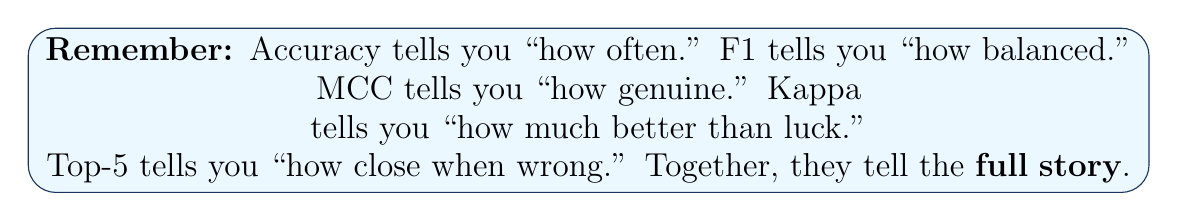
\begin{tikzpicture}
\node[draw=darkblue, fill=lightblue, rounded corners=10pt, text width=14cm, align=center, minimum height=2cm, font=\large] {
    \textbf{Remember:} Accuracy tells you ``how often.'' F1 tells you ``how balanced.''\\
    MCC tells you ``how genuine.'' Kappa tells you ``how much better than luck.''\\
    Top-5 tells you ``how close when wrong.'' Together, they tell the \textbf{full story}.
};
\end{tikzpicture}
\end{center}

\end{document}
